\section{Mind Map Searching}
\label{prototype:MapSearching}
Another key aspect of my software is the ability to search through the notes and tags you create. Whilst I placed a search box at the top of my prior iteration this wasn’t yet functional, that now changes.

With some small code changes on the front and backend it is now possible to search through notes, clicking the background returns the user to the all notes view

\begin{figure}[H]
    \centering
    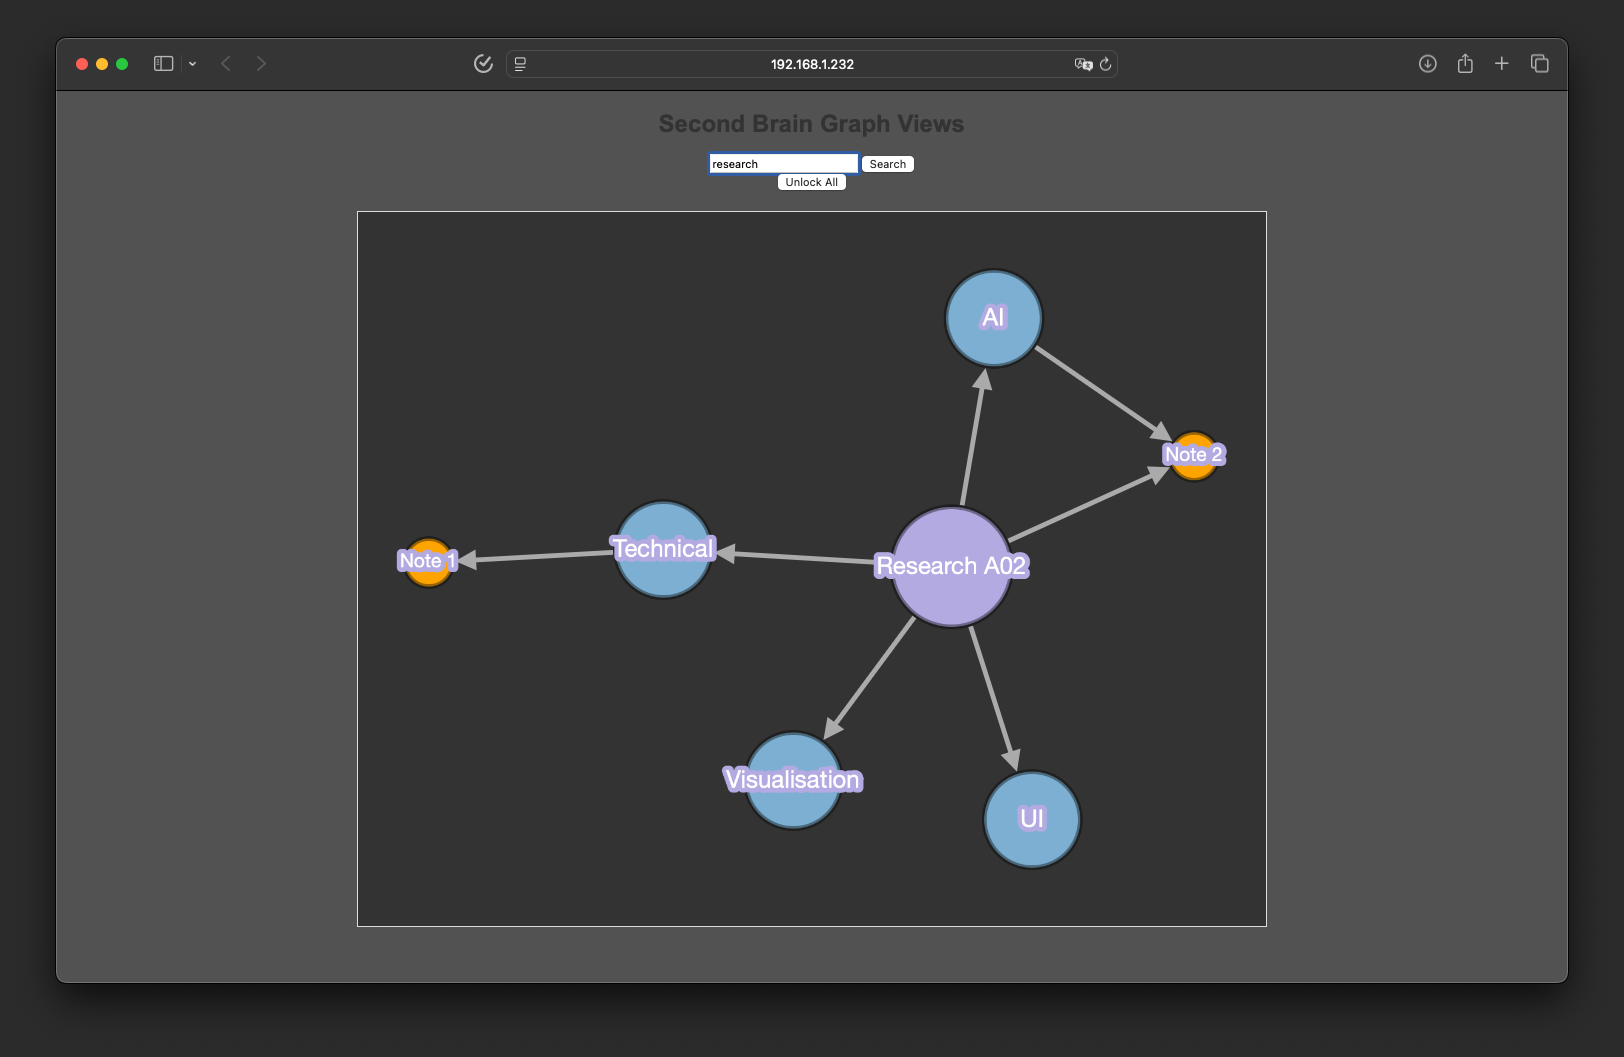
\includegraphics[width=0.8\textwidth]{Prototype/8_MapSearching/media/prototype.png}
    \caption{Search Functionality}
\end{figure}

\textbf{Code:}
Backend - adding a new route which the front end can call with a search query:
\inputminted[linenos, tabsize=1, breaklines]{py}{prototype/8_MapSearching/media/backend.py}

Frontend - adding a function to send the search form content to the backend when entered, and then updating the graph shown:
\inputminted[linenos, tabsize=1, breaklines]{js}{prototype/8_MapSearching/media/frontend.js}